\section{Trees, Binomial random variables, independence} \label{s2} 

\ssn{Learning outcomes}
After studying this week you will be able to: 
\begin{itemize}
\item Use probability trees to calculate probabilities
\item Solve problems using the binomial distribution
\item Be able to explain and to use random variables and their expectations.
\end{itemize}
\end{n}  

\subsection{Preparation for the week} 

\ssn{Motivating problems} \label{mp2}
\begin{itemize}
    \item A production line produces components and it is assumed that each component independently has a probability $0.05$ of being faulty. Ten random samples are taken of the product; what is the probability that two or more are faulty? 
 \item A multiple choice test has ten questions, each having four possible answers. A student randomly guesses which answer is correct for every question.  What is the probability that they get an `A' by answering at least seven correctly? 
\end{itemize}
A little though should convince you that these problems are essentially the same: they are asking how likely we are to succeed $k$ times out of $n$ if each of the $n$ trials independently has probability $p$ of success. 
\end{n}


\ssn{How many `6's in three rolls?}
If I roll a D6 three times, what is the probability of three `6's? This is one outcome of the $6^3=216$ equally likely outcomes and so has probability $1/216$. 

Alternatively, we can think in stages. The probability of the first roll being `6' is $1/6$. The probability of the second roll then also being a `6' is $1/6$ and so the probability of the first two rolls being `6's is $(1/6)\times(1/6) = 1/36$. Finally, the probability of the third roll being a `6' is $1/6$ and so the probability of all three being `6's is $(1/6)^3 = 1/216$. 
We can sum this calculation up in a \emph{probability tree}: 

\tikzset{
  treenode/.style = {shape=rectangle, rounded corners,
                     draw, align=center, 
                     top color=white, bottom color=blue!30},
  root/.style     = {treenode, font=\Large, bottom color=red!30},
  env/.style      = {treenode},
  branch/.style = {treenode, bottom color=blue!10},  
  dummy/.style    = {circle,draw}
}
\tikzstyle{level 1}=[level distance=3.5cm, sibling distance=3.5cm]
\tikzstyle{level 2}=[level distance=3.5cm, sibling distance=2cm]

\begin{center}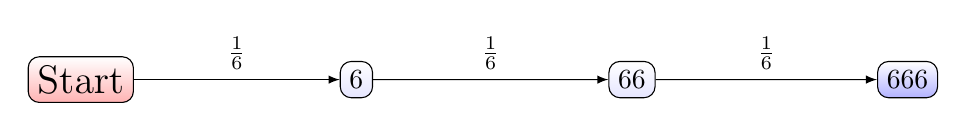
\begin{tikzpicture}
[
grow=right,
    edge from parent/.style = {draw, -latex},
    every node/.style       = {font=\normalsize}
  ]
\node[root]{Start}
child {
    node[branch]{6}
    child {
        node[branch]{66}
        child {
            node[env]{666}
            edge from parent node[above] {$\frac{1}{6}$}                      }
        edge from parent node[above] {$\frac{1}{6}$}
        }                
    edge from parent node[above] {$\frac{1}{6}$}        
    }  ;           
\end{tikzpicture}
\end{center} 
\smallskip 
You may feel this tree has fewer branches than a good tree should have. Of course, other things could happen along the way which we have omitted. All the branches appear in the full tree in Table~\ref{bigtree}, where we write `x' for a roll that is not a `6'.  

\begin{table}[h] 
\tikzstyle{level 1}=[level distance=3.5cm, sibling distance=5.0cm]
\tikzstyle{level 2}=[level distance=3.5cm, sibling distance=2.5cm]
\tikzstyle{level 3}=[level distance=3.5cm, sibling distance=1.3cm]

\begin{center} 
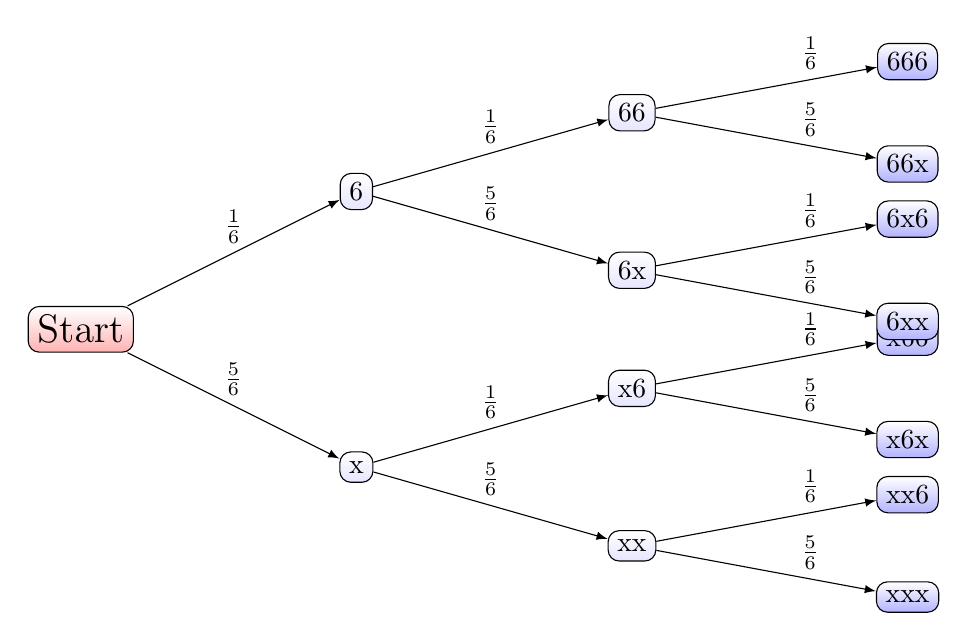
\begin{tikzpicture}
[
grow=right,
    edge from parent/.style = {draw, -latex},
    every node/.style       = {font=\normalsize}
  ]
\node[root]{Start}
child { 
    node[branch]{x}
    child { 
        node[branch]{xx}
        child{ 
             node[env]{xxx}
             edge from parent node[above,pos=0.7]{$\frac{5}{6}$}                    }
        child{ 
             node[env]{xx6}
             edge from parent node[above,pos=0.7]{$\frac{1}{6}$}      
             }               
        edge from parent node[above]{$\frac{5}{6}$} 
        }       
    child { 
        node[branch]{x6}
        child{ 
             node[env]{x6x}
             edge from parent node[above,pos=0.7]{$\frac{5}{6}$}                    }
        child{ 
             node[env]{x66}
             edge from parent node[above,pos=0.7]{$\frac{1}{6}$}      
             }               
        edge from parent node[above]{$\frac{1}{6}$} 
        }       
    edge from parent node[above]{$\frac{5}{6}$}            
    }
child { 
    node[branch]{6}
    child { 
        node[branch]{6x}
        child{ 
             node[env]{6xx}
             edge from parent node[above,pos=0.7]{$\frac{5}{6}$}                    }
        child{ 
             node[env]{6x6}
             edge from parent node[above,pos=0.7]{$\frac{1}{6}$}      
             }               
        edge from parent node[above]{$\frac{5}{6}$} 
        }       
    child { 
        node[branch]{66}
        child{ 
             node[env]{66x}
             edge from parent node[above,pos=0.7]{$\frac{5}{6}$}                    }
        child{ 
             node[env]{666}
             edge from parent node[above,pos=0.7]{$\frac{1}{6}$}      
             }               
        edge from parent node[above]{$\frac{1}{6}$} 
        }       
    edge from parent node[above]{$\frac{1}{6}$}            
    }     ;           
\end{tikzpicture} \end{center} 
\caption{Rolling a die 3 times and seeing how many `6's occur. \label{bigtree}} 
\end{table} 
\end{n}

\ssn{Using the tree}
In the tree in Table~\ref{bigtree}, the probability of an outcome is the product of the probabilities along the path leading to it.  The probability of rolling `x6x' is thus 
 \[
     \frac56 \; \frac16 \; \frac56 = \frac{25}{216}. 
 \]
 
 We could ask, for instance what is the probability of the event $A$ of getting two sixes in a row at some point in our three rolls. There are three branches of the tree with this property and adding we get 
  \[
 \PP(A) = \frac16\;\frac16 \; \frac16 + 
  \frac16\;\frac16 \; \frac56 +
    \frac56\;\frac16 \; \frac16  = \frac{11}{216}. 
  \]
Here we have used the fact that probabilities for 
disjoint events (getting two `6's in the three different ways) add. 
\end{n}


\ssn{Another tree example} 
In Workshop~1 we calculated the win probability for Blue when rolling two six sided dice: Blue numbered $(6,3,3,3,3,3)$ versus Green numbered $(5,5,5,2,2,2)$. 

If we imagine Blue rolling first, we can draw a tree as below. 

\tikzset{
  treenode/.style = {shape=rectangle, rounded corners,
                     draw, align=center, 
                     top color=white, bottom color=blue!30},
  root/.style     = {treenode, font=\Large, bottom color=red!30},
  env/.style      = {treenode},
  branch/.style = {treenode, bottom color=blue!10},  
  dummy/.style    = {circle,draw}
}
\tikzstyle{level 1}=[level distance=3.5cm, sibling distance=3.5cm]
\tikzstyle{level 2}=[level distance=3.5cm, sibling distance=2cm]

\begin{center}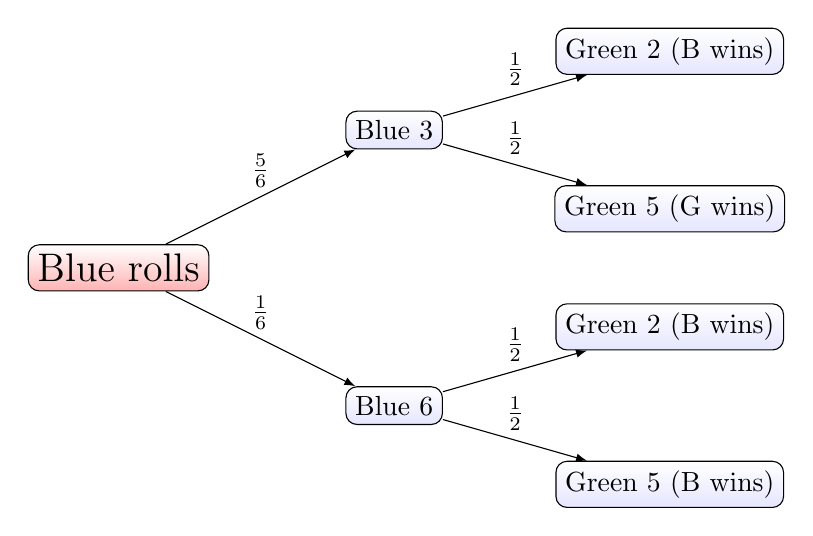
\begin{tikzpicture}
[
grow=right,
    edge from parent/.style = {draw, -latex},
    every node/.style       = {font=\normalsize}
  ]
\node[root]{Blue rolls}
child {
    node[branch]{Blue 6}
    child {
        node[branch]{Green 5 (B wins)}
        edge from parent node[above] {$\frac{1}{2}$}
        }  
    child {
        node[branch]{Green 2 (B wins)}
        edge from parent node[above] {$\frac{1}{2}$}
        }  
    edge from parent node[above] {$\frac{1}{6}$}        
    }     
child {
    node[branch]{Blue 3}
    child {
        node[branch]{Green 5 (G wins)}
        edge from parent node[above] {$\frac{1}{2}$}
        }  
    child {
        node[branch]{Green 2 (B wins)}
        edge from parent node[above] {$\frac{1}{2}$}
        }   
    edge from parent node[above] {$\frac{5}{6}$}        
    }  ;    
\end{tikzpicture}
\end{center} 
There is a single path to a Green win and that has probability $(5/6)(1/2) = 5/12$.  So blue wins with probability $1 - (5/12) = 7/12$. 

You could observe that Blue has certainly won if they roll a `6' and so one could terminate the lower branch at that point.  
\end{n} 
